\documentclass{beamer}
\usepackage[absolute,overlay]{textpos}
\usepackage{fancybox}
\useinnertheme{rectangles}
\setbeamercovered{transparent}
\usepackage{amsmath}
\usepackage{graphicx}
%\usepackage{multimedia}
\usepackage{hyperref}
\usepackage{movie15}
\newcommand{\LaunchBinary}[2]{%
  % #1: layer name,
  % #2: link text
  \leavevmode%
  \pdfstartlink user {
    /Subtype /Link
    /Border [0 0 0]%
    /A <<
      /F <<
         /DOS (xxx)
         /Unix (#1)
         /Mac (xxx)
      >>
      /S /Launch
    >>
  }#2%
  \pdfendlink%
}
\mode<presentation>
{
  \usetheme{CambridgeUS}%{PaloAlto}%Marburg}
  % or ...
\usecolortheme{seagull}%dove}%{seahorse}
  \setbeamercovered{transparent}
  % or whatever (possibly just delete it)
}


\usepackage[english]{babel}
% or whatever

\usepackage[latin1]{inputenc}
% or whatever

\usepackage{times}
\usepackage[T1]{fontenc}
\title[UW]% (optional, use only with long paper titles)
{\textbf{Ocean model utility and horizontal resolution:\\\small A Southern Ocean case study}}
\vspace{-0.5cm}
\date[1st Jul. 2016]{1st July 2016}

\subject{Talks}
\author[maike\_s@mit.edu]
{
  \textcolor{green!50!black}{Maike~Sonnewald}\inst{1} \and
  Jo\"{e}l J.-M. Hirschi\inst{2} \and
  James Dyke\inst{3} \and\\
  George A. Nurser\inst{2} \and
}

\institute[]
{
  \inst{1}%
  Dept. of Earth, Atmospheric and Planetary Sciences,\\
  Massachusetts Institute of Technology, USA
  \and
  \vskip-2mm
  \inst{2}%
  National Oceanography Center, Southampton,
  University of Southampton, UK
  \and
  \vskip-2mm
  \inst{3}%
  Institute for Complex Systems Simulation,
  University of Southampton, UK
  \vskip-1mm
  \begin{columns}[c]
  \column{1.2in}
  \centering
  
\includegraphics[width=0.65\textwidth]{mitLogo.jpg}%
  \column{1.7in}
  \centering
  
\includegraphics[width=1\textwidth]{logoNOCS.png}%
  \column{2in}
  \centering
  
\includegraphics[width=0.55\textwidth]{icss_logo.png}%
  \end{columns}
}



\begin{document}


% \insertpagenumber
\begin{frame}
  \titlepage
\end{frame}


\begin{frame}{Outline}
\begin{columns}[c]
\column{2in}
  \tableofcontents%[pausesections]
%  You might wish to add the option [pausesections]
\column{2in}
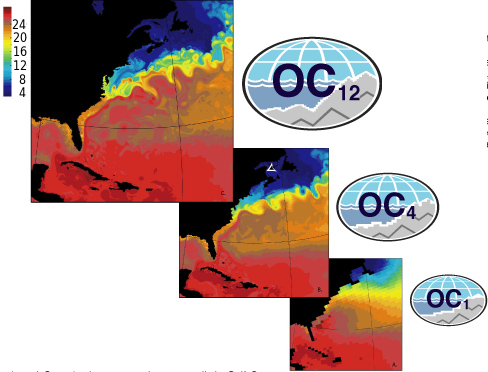
\includegraphics[width=1\textwidth]{occam.png}\\
\end{columns}
\vspace{0.52cm}
\begin{alertblock}{Systematic assessment of changes with ocean model resolution}
    \centering Take home: Different resolutions suitable for different applications!
\end{alertblock}
\end{frame}

\begin{frame}{Motivation}
 \begin{columns}[c]
\column{1.5in}
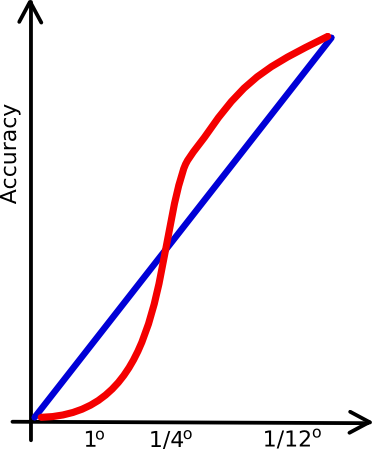
\includegraphics[width=1\textwidth]{accuracy_rez.png}\\
\column{3in}
\begin{itemize}
 \item Really big, hard, question!% We do not try to address this in its entirety!
 \item What resolution is ``good enough''?
 \item IPCC -> Drive towards higher resolution. Is it worth it?
 \item Low resolution is faster, easier, cheaper...
\end{itemize}
\end{columns}
\pause
\begin{alertblock}{Boundary layers key}
    \centering Southern Ocean case studies: Bathymetry interactions and Mixed Layer Depth
\end{alertblock}
\end{frame}


\begin{frame}{Where should we look for changes?}
\begin{center}
\begin{columns}[c]
\column{1.7in}
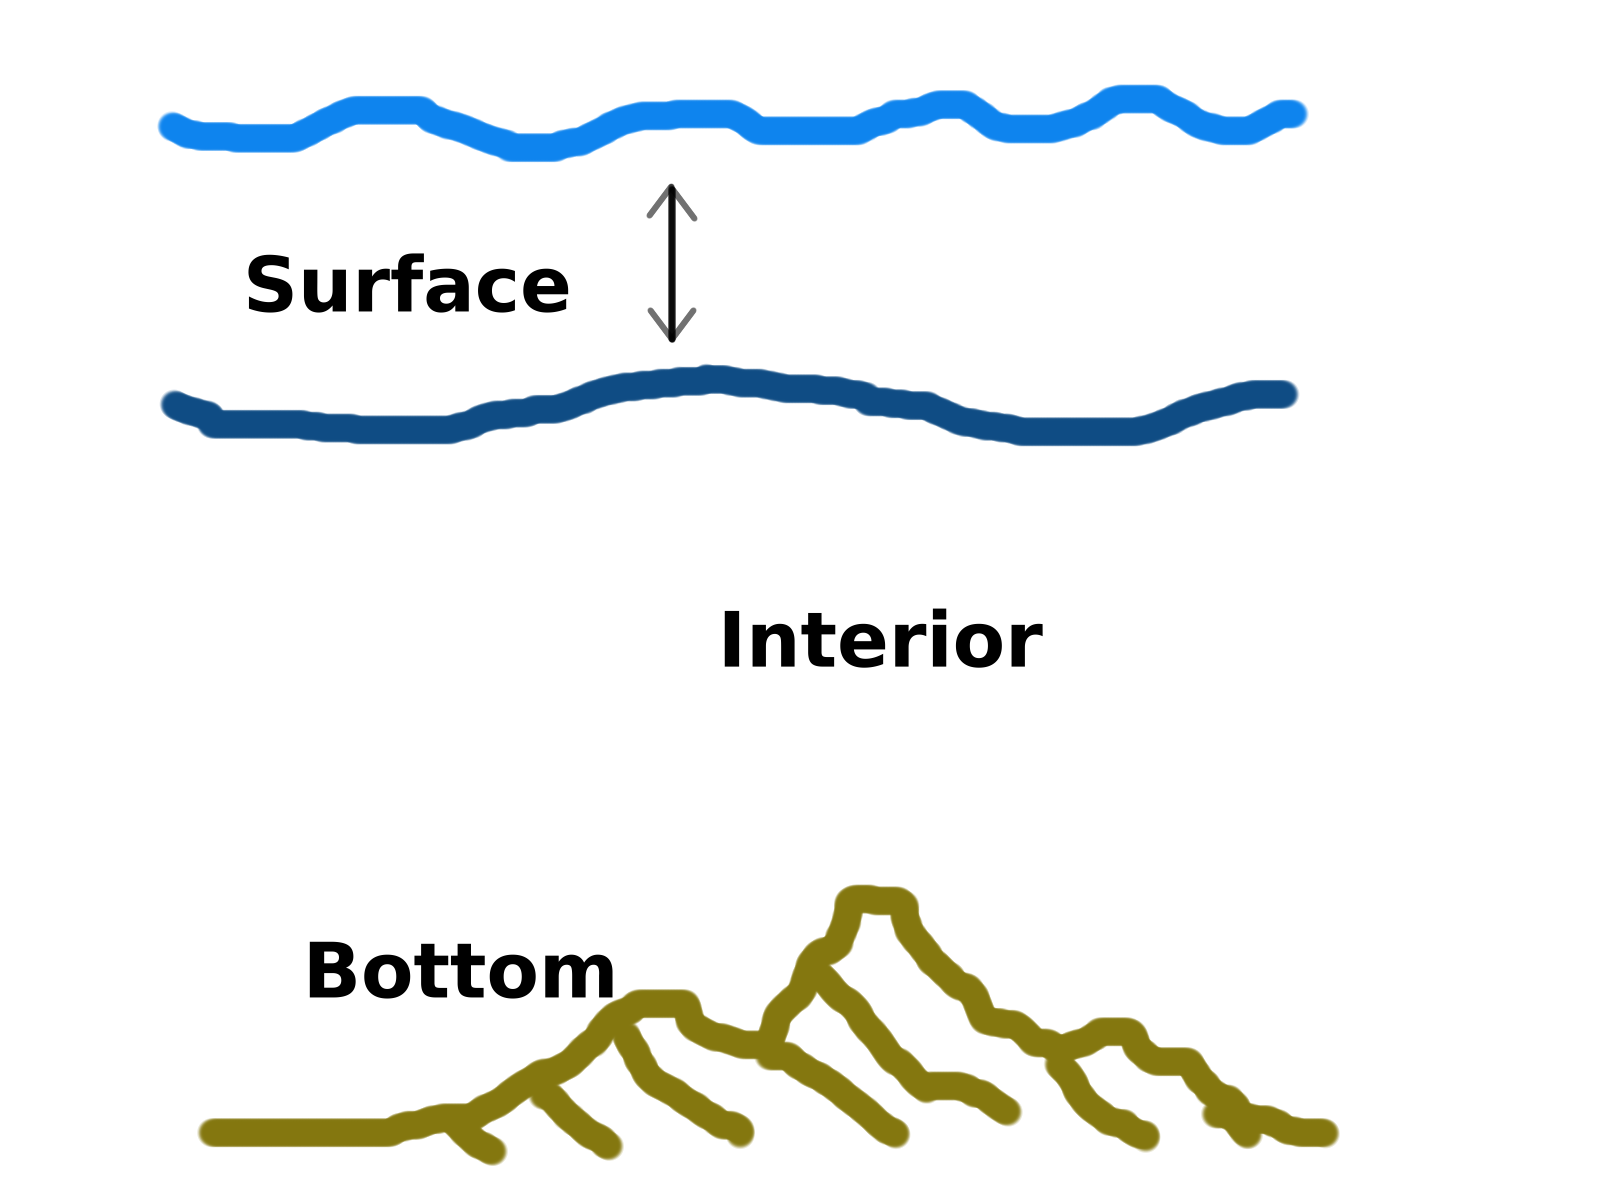
\includegraphics[width=1.5\textwidth]{momSink.png}
\column{1.7in}
\pause
\begin{enumerate}
 \item Mixed Layer Depth
 \item Steric height
 \item Bottom interactions
\end{enumerate}

\end{columns}
\end{center}
%\vspace{2cm}
%We look at the \textbf{surface}, \alert{Interior} and \alert{deep} as places where the ocean could change.
\begin{alertblock}{Depth-integrated momentum equation:}
 $$f \mathrm{\textbf{k}} \times \mathrm{\textbf{U}} + \nabla P  = p_{b}\nabla H + \tau_{w} - \tau_{b} - \mathrm{\textbf{R}},$$
\end{alertblock}
\end{frame}




\section{The model: NEMO}

\begin{frame}{\textbf{N}ucleus of \textbf{E}uropean \textbf{M}odelling of the \textbf{O}cean:\\\textbf{NEMO} (Madec, 2008)}

\begin{center}
\LaunchBinary{The_NEMO_global_ocean_model_720p.mp4}{
\includegraphics[width=0.4\textwidth]{Logo_NEMO.png}}%{Start ORCA12 surface currents}
\end{center}
\vspace{0.5cm}
\begin{alertblock}{}
    \centering Suite of realistic GCM runs from 1978-2007\\forced with DFS4.1 (Brodeau \textit{et al.}, 2010) 
\end{alertblock}
\end{frame}

\begin{frame}{What parameters change with resolution?}

\begin{table}
\scalebox{0.7}{
 \begin{tabular}{|c |c | c | c |}
    \hline
    Name & ORCA1-N406 & ORCA025-N401 & ORCA0083-N01\\ 
    Resolution & 1$^{\circ}$&1/4$^{\circ}$&1/12$^{\circ}$\\ \hline
    z, x, y& 75,292,362 & 75,1021,1442 & 75,3059,4322 \\ 
    GM active &Yes & No & No \\
    Horiz. laplacian eddy viscosity ($m^{2}s^{-1}$)& $10^{4}$&500 &500 \\
    Horiz. bilaplacian eddy viscosity ($m^{4}s^{-1}$)& $-1.25\times 10^{10}$&$-2.2\times 10^{11}$ &$-2.2\times 10^{11}$ \\
    Isopycnal eddy tracer diffusivity ($m^{2}s^{-1}$)& $10^{3}$&300 & 125\\
    Timestep ($s$)& 3600& 1440 & 200 \\
    \hline
\end{tabular}}
    %\caption{A collection of metrics for the NEMO resolutions.}
    %\label{NEMO_stats}
\end{table}
\begin{alertblock}{}
    \centering Runs were designed by Andrew Coward and Beverly de Cuevas to be as comparable as feasible 
\end{alertblock}
\end{frame}


%\section{Metrics and ``Utility''}

\begin{frame}{Tools for comparing the model runs}
\begin{columns}[c]
\column{1.7in}
 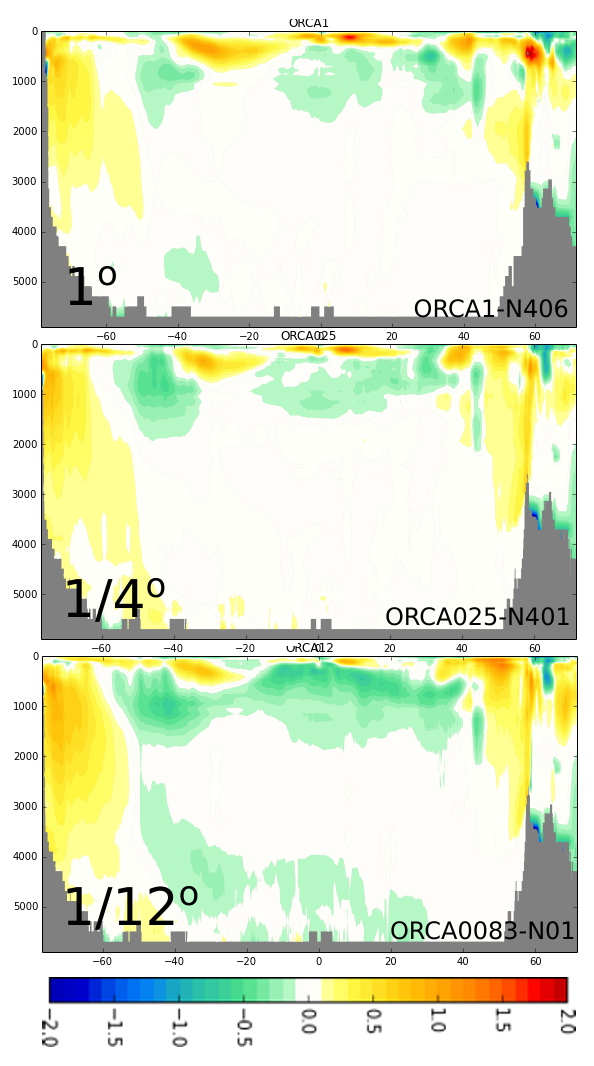
\includegraphics[width=1\textwidth]{MOC_biasPrez2.png}\\
 %$\psi(z, y)$: Depth-latitude streamfunction EN3 bias ($^{o}$C) (Hyder \textit{et al.}, In Prep.)
 %\includegraphics[width=1.15\textwidth]{/home/maike/Documents/thesis/reynoldsSSTbiasPrez.jpg}
\column{3in}
\begin{itemize}
 \item Changes compared to observations
 \item $\psi(z, y)$: Depth-latitude streamfunction EN3 bias ($^{o}$C) \small (Hyder \textit{et al.}, In Prep.)
 \begin{itemize}
  \item Do these changes ``matter''?
  \item When/where? Is cost \alert{merited}?
 \end{itemize}
 \item We use area averaged PDF% and finite-time Lyapunov exponents (FTLE, not presented)
% \item We also explore ``utility'', more on this later...
\end{itemize}
\end{columns}
\end{frame}




%\begin{frame}{$\psi(z, y)$: Depth-latitude streamfunction EN3 bias ($^{o}$C)}
%\begin{center}
% \includegraphics[width=1\textwidth]{/home/maike/Documents/thesis/MOC_biasPrez.png}\\
% (Hyder \textit{et al.}, In Prep.)
%\end{center}
%\end{frame}



\begin{frame}{Introduction: Bathymetry interactions}
\begin{columns}[c]
\column{3in}
\centering
\begin{alertblock}{}
\begin{center}
\begin{itemize}%Using the laminar view of the ocean, we can look at 
  \item \small \alert{Southern Ocean} zonal pressure/buoyancy gradients \alert{not} balanced by topography
  \vspace{15}
  \item \small Non-linear eddy terms become important 
  \vspace{15}
  \item \small Southern Ocean is key climatically 
\end{itemize}
\end{center}
\end{alertblock}
\column{2in}

\begin{flushright}
\includegraphics[width=1\textwidth]{/home/maike/Documents/EGU2015/NEMOwLogo.png}\end{flushright}
\end{columns}
\pause
\begin{alertblock}{Question:}
\centering
 \alert{How do balance of forces expressed through $J(p_{b}, H)$ change with \alert{resolution}?}
\end{alertblock}
\end{frame}

\begin{frame}{Introduction: Bathymetry interactions}
\begin{columns}[c]
\column{3in}
\centering
%\begin{alertblock}{}
\begin{center}
\begin{itemize}%Using the laminar view of the ocean, we can look at 
  \item Ocean heat fluxes important for \alert{climate}
  \item Gyre circulation, geostrophic f/H contours:
  \small$\beta \psi_{x}=\overbrace{-f w_{B}}^{\text{vertical bottom vel.}}+\underbrace{\nabla \times \tau}_{\text{wind stress}} + \overbrace{R'}^{\text{Non-lin terms}}$ \\
  \vspace{15}
  \item Interactions with \alert{bathymetry}:
    $w_{B} = u_{B}\cdot \nabla (-H) = \frac{1}{\rho_{0}f}J(p_{B}, -H)$
  \item Bathymetry can profoundly influence model behaviour; \alert{Horizontal resolution}
\end{itemize}
\end{center}
%\end{alertblock}
\column{2in}

\begin{flushright}
\includegraphics[width=1\textwidth]{/home/maike/Documents/EGU2015/marshallSpeer.jpg}\\
\tiny Marshall and Speer (2012)\end{flushright}
\end{columns}
\end{frame}




\begin{frame}{Density-latitude streamfunction ($\psi(\sigma, y)$): Definition}
Illustrating the heat transport in the system: 
\vspace{-0.5cm}
\begin{flushright} \tiny Zika \textit{et al.} (2012), Nurser and Lee (2004)\end{flushright}
%\begin{columns}[c]
%\column{2.5in}
\vspace{-1.5cm}
\centering
\begin{center}
\large
\begin{equation*}
\huge \psi(\sigma, y) = \int \int_{\sigma*<\sigma}v(x,y,z)dzdx
\end{equation*}
\end{center}

%column{2.5in}
%\begin{flushleft}
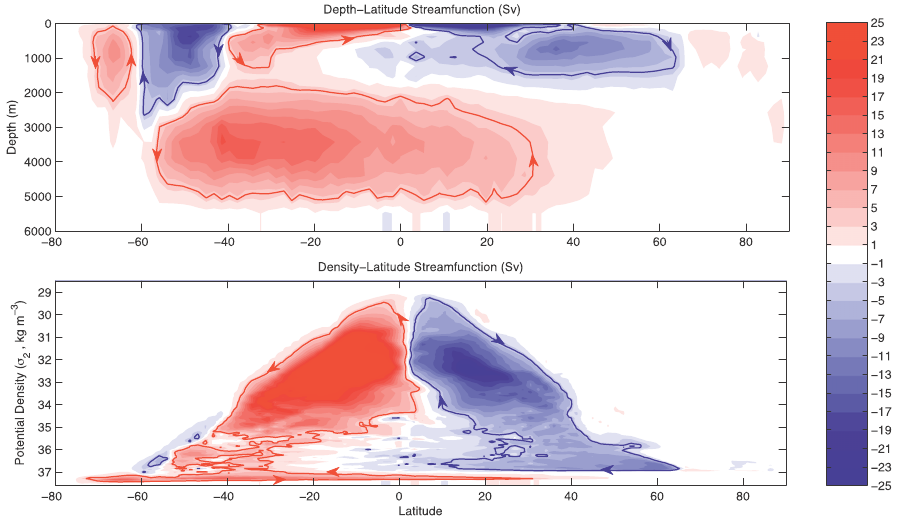
\includegraphics[width=0.8\textwidth]{zikaOverturning.png}\\


%\end{flushleft}
%\begin{flushright}\

%\end{flushright}
%\end{columns}
%\tiny 
\end{frame}
%title
%MLD equation
% More labels
%Context: How much is high enough? Levy

\begin{frame}{Density-latitude streamfunction ($\psi(\sigma, y)$): Interpretation}
\begin{center}
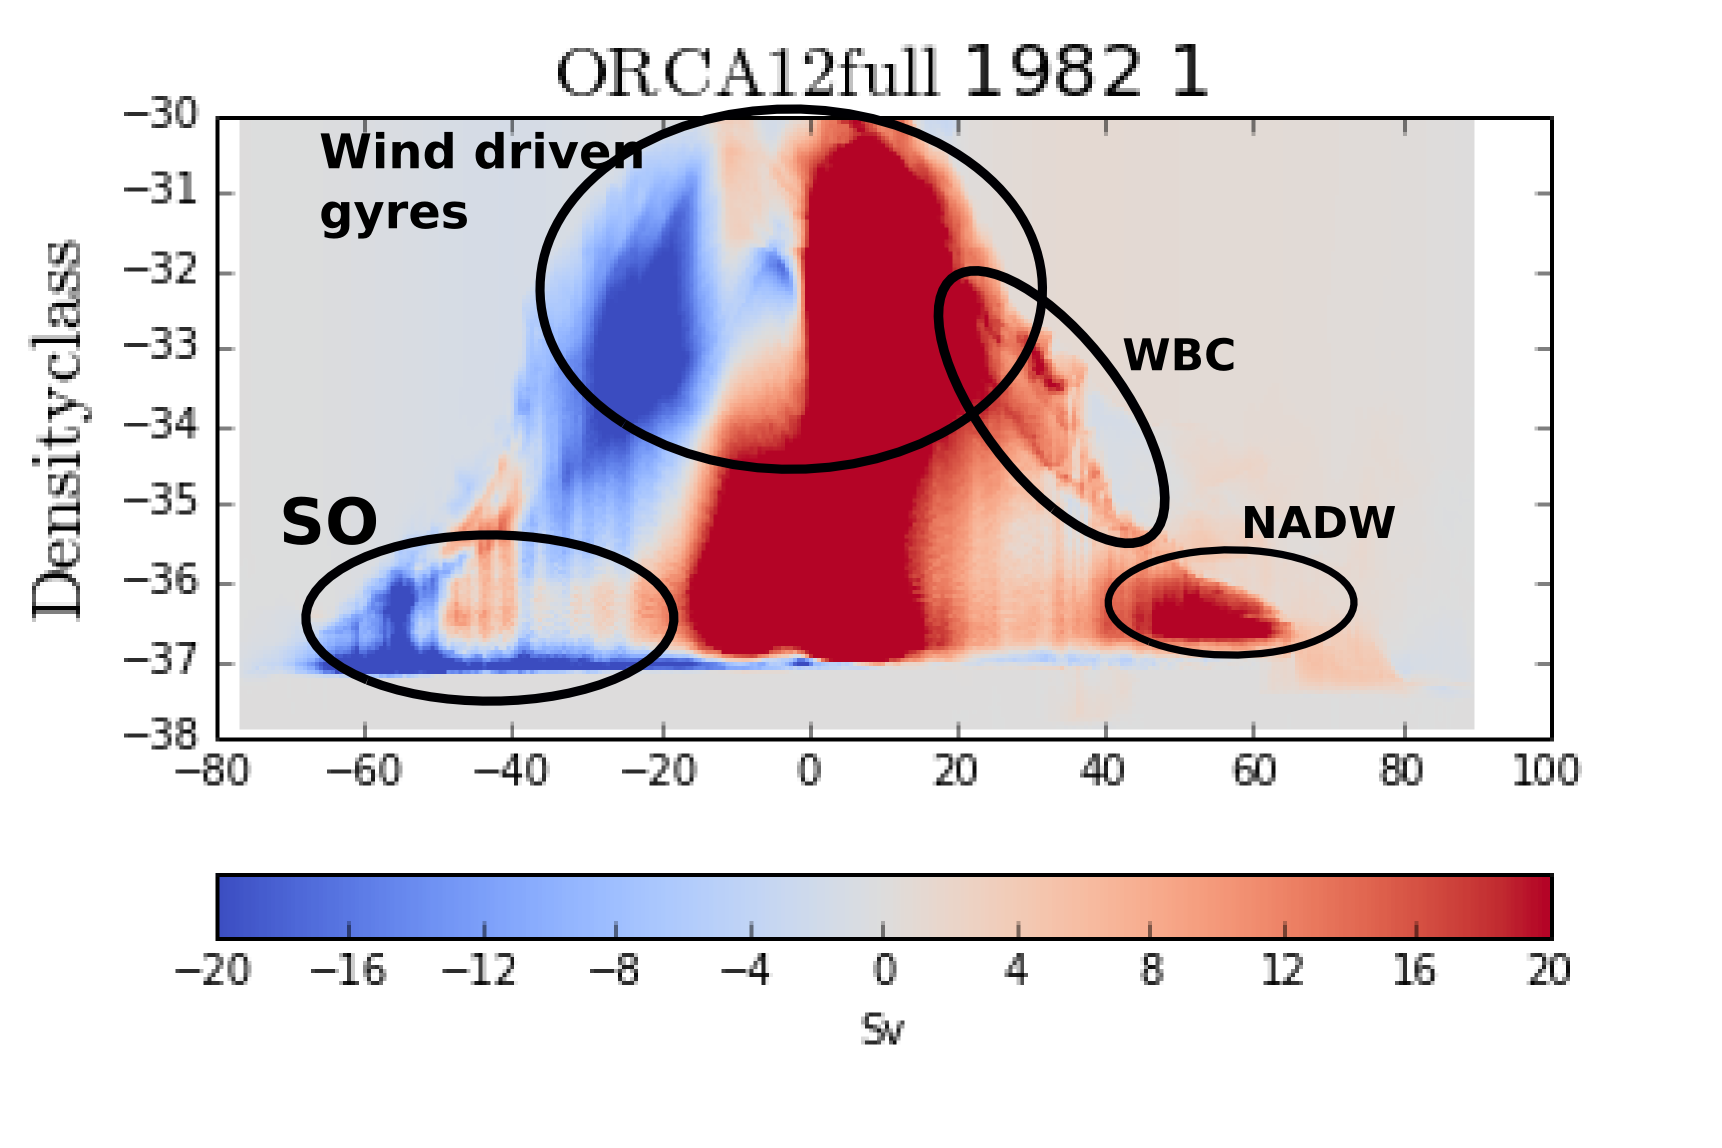
\includegraphics[width=1\textwidth]{demoPsi.png}
\end{center}
\end{frame}

\begin{frame}{Density-latitude streamfunction ($\psi(\sigma, y)$):\\Mean 1978-2007}
\vspace{-0.4cm}
\begin{figure}[H]
\centering
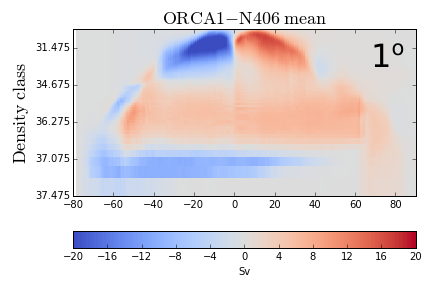
\includegraphics[width=0.5\textwidth]{mocsigORCA1_fullMeanStreatchedP.png}
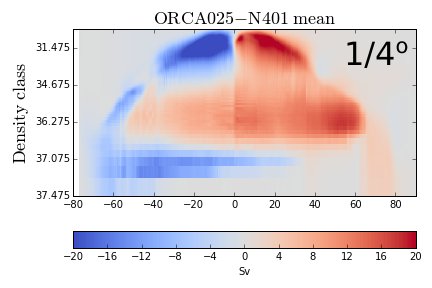
\includegraphics[width=0.5\textwidth]{mocsigORCA025_fullMeanStreatchedP.png}\\
\vspace{-0.2cm}
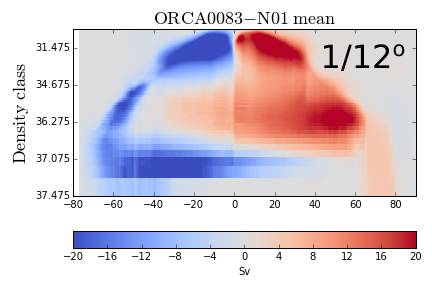
\includegraphics[width=0.5\textwidth]{mocsigORCA12_fullMeanStreatchedP.png}

\end{figure}
\end{frame}

%Full mergedmocsigORCA12_baroc_300.png
\begin{frame}{Density-latitude streamfunction ($\psi(\sigma, y)$): Transient}
\begin{center}
\LaunchBinary{mocsigORCA1_12_full_short.avi}{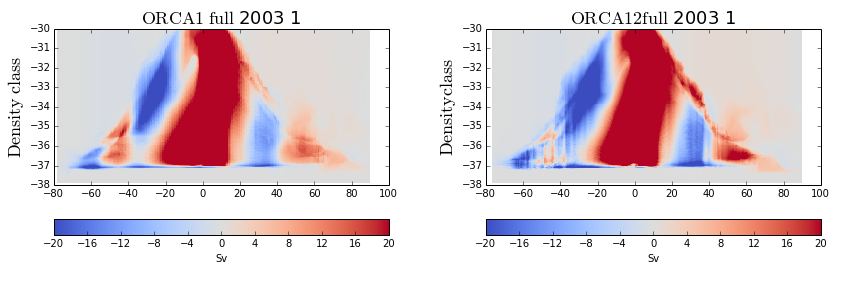
\includegraphics[width=1\textwidth]{mergedmocsigORCA12_full_300.png}}%{Start ORCA12 surface currents}
\end{center}
\end{frame}

\begin{frame}{The barotropic ($\overline{\psi}$) and baroclinic ($\psi'$) decomposition}
\begin{center}
\huge $$\psi_{\sigma y} &= \overline{\psi}_{\sigma y} + \psi'_{\sigma y}$$
\centering 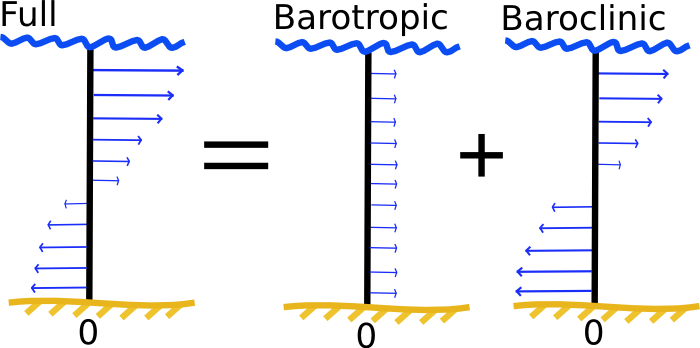
\includegraphics[width=0.6\textwidth]{baroCT.png}
\end{center}
\end{frame}

\begin{frame}{$\overline{\psi}(\sigma, y)$: Barotropic streamfunction}
%\vspace{-0.5cm}
%\small The barotropic ($\overline{\psi}$) and baroclinic ($\psi'$) decomposition: \huge $\psi_{\sigma y} &= \overline{\psi}_{\sigma y} + \psi'_{\sigma y}$
% \begin{center}
% \vspace{-30}
% \huge
% \begin{equation*}
%  
% \end{equation*}
% \end{center}
 \begin{figure}[H]
 %\vspace{-25}
\centering
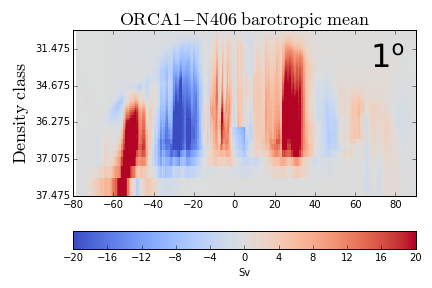
\includegraphics[width=0.5\textwidth]{mocsigORCA1_barotMeanStreatchedP.png}
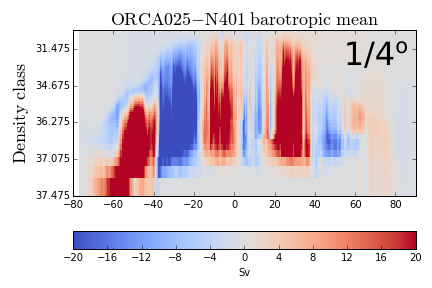
\includegraphics[width=0.5\textwidth]{mocsigORCA025_barotMeanStreatchedP.png}\\
\vspace{-0.2cm}
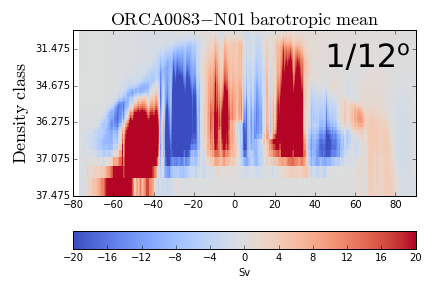
\includegraphics[width=0.5\textwidth]{mocsigORCA12_barotMeanStreatchedP.png}

%   \caption{\normalsize The overturning in $\rho$ space. Showing the mean barotropic and baroclinic circulation from the 1978 to 2007 timeseries.}
%   \label{mocsigBarotBaroc}
\end{figure}
\end{frame}

\begin{frame}{$\psi'(\sigma, y)$:Baroclinic streamfunction}
 \begin{figure}[H]
 %\vspace{-25}
\centering
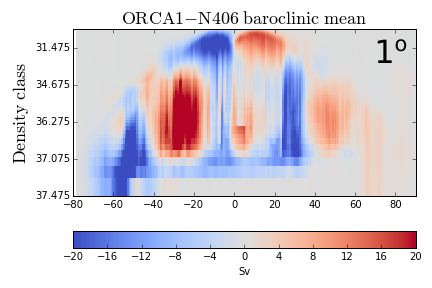
\includegraphics[width=0.5\textwidth]{mocsigORCA1_barocMeanStreatchedP.png}
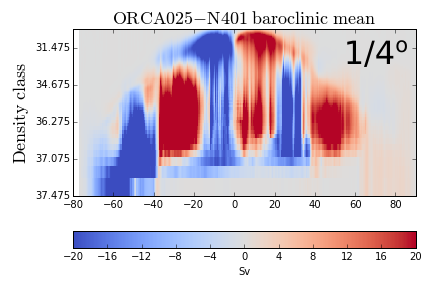
\includegraphics[width=0.5\textwidth]{mocsigORCA025_barocMeanStreatchedP.png}\\
\vspace{-0.2cm}
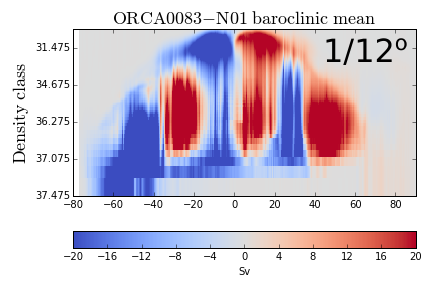
\includegraphics[width=0.5\textwidth]{mocsigORCA12_barocMeanStreatchedP.png}

%   \caption{\normalsize The overturning in $\rho$ space. Showing the mean barotropic and baroclinic circulation from the 1978 to 2007 timeseries.}
%   \label{mocsigBarotBaroc}
\end{figure}
\end{frame}

\begin{frame}{1/12$^{\circ}$: Eddy compensation?\tiny Farneti \textit{et al.} (2010), Hallberg and Gnanadesikan (2006)}
 \begin{figure}[H]
 %\vspace{-25}
\centering
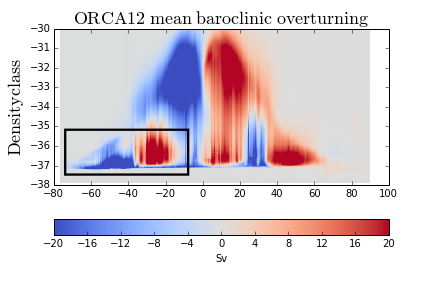
\includegraphics[width=0.5\textwidth]{mocsigORCA12MeanBaroc_BOX.png}
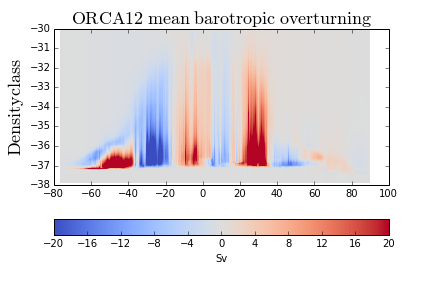
\includegraphics[width=0.5\textwidth]{mocsigORCA12MeanBarot.png}\\
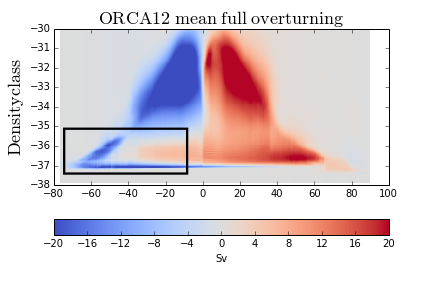
\includegraphics[width=0.5\textwidth]{mocsigORCA12MeanFull_BOX.png}
%\caption{\normalsize The overturning in $\rho$ space. Showing the mean barotropic and baroclinic circulation from the 1978 to 2007 timeseries.}
%   \label{mocsigBarotBaroc}
\end{figure}
\begin{alertblock}{}
 Suggestive of eddy compensation? \tiny Farneti \textit{et al.} (2010), Hallberg and Gnanadesikan (2006)
\end{alertblock}
\end{frame}








\section{Surface: Mixed Layer Depth}
\begin{frame}{The mixed layer: Schematic}
\begin{figure}
\center 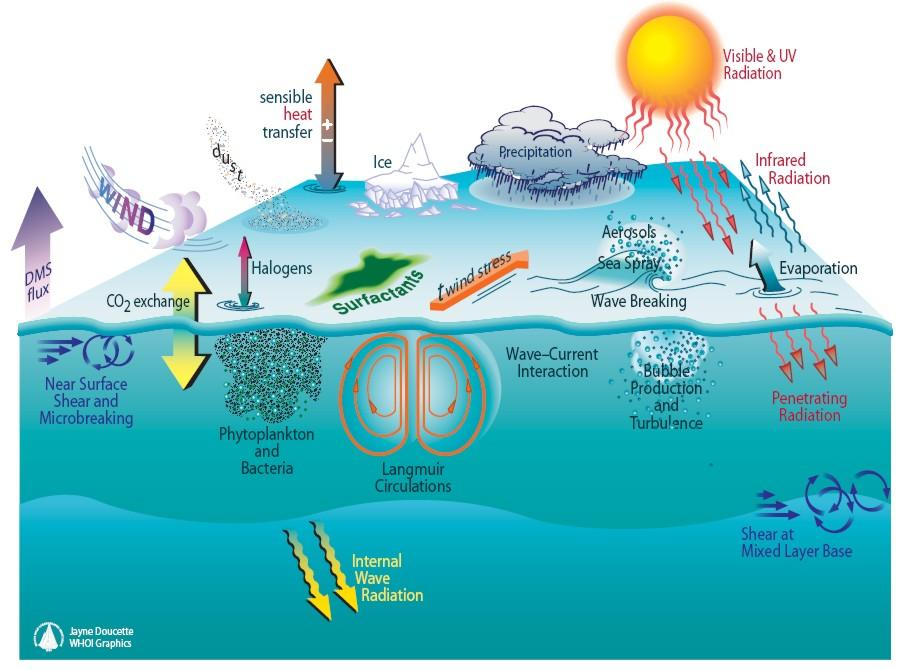
\includegraphics[width=0.7\textwidth]{mixed_layer_schematic.png}
\end{figure}
\tiny Image from:$http://www.ifremer.fr/cerweb/deboyer/mld/SurfaceMixedLayerDepth.php$
\end{frame}

\begin{frame}{MLD (m) climatology movie, 1978-2007}
%\begin{center}
%\LaunchBinary{/home/maike/Documents/nemo/MLD/ORCA1/mld_ORCA1_clim_online.avi}{\includegraphics[width=0.5\textwidth]{/home/maike/Documents/nemo/MLD/ORCA1/mld_ORCA1_clim_m06.png}}%{Start ORCA12 surface currents}
\LaunchBinary{/home/maike/Documents/nemo/MLD/ORCA12/mld_ORCA12_clim_online.avi}{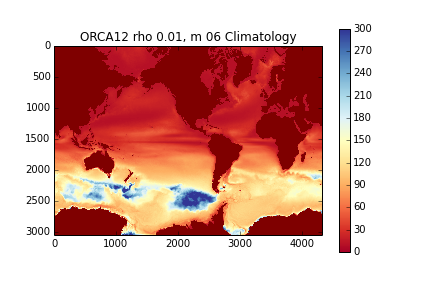
\includegraphics[width=0.5\textwidth]{mld_ORCA12_clim_m06.png}}\LaunchBinary{mld_ORCA1_clim_online.avi}{\includegraphics[width=0.5\textwidth]{mld_ORCA1_clim_m06.png}}
%\end{center}
\begin{alertblock}{MLD criterion }
\centering $\Delta \rho = 0.03 kg m^{-3}$, $ \Delta \rho = |\mathrm{\rho}_{s}-\mathrm{\rho}_{d}| $
\end{alertblock}

\end{frame}

\begin{frame}{January and September MLD PDFs}
\vspace{-0.5cm}
 \begin{figure}
  \center
	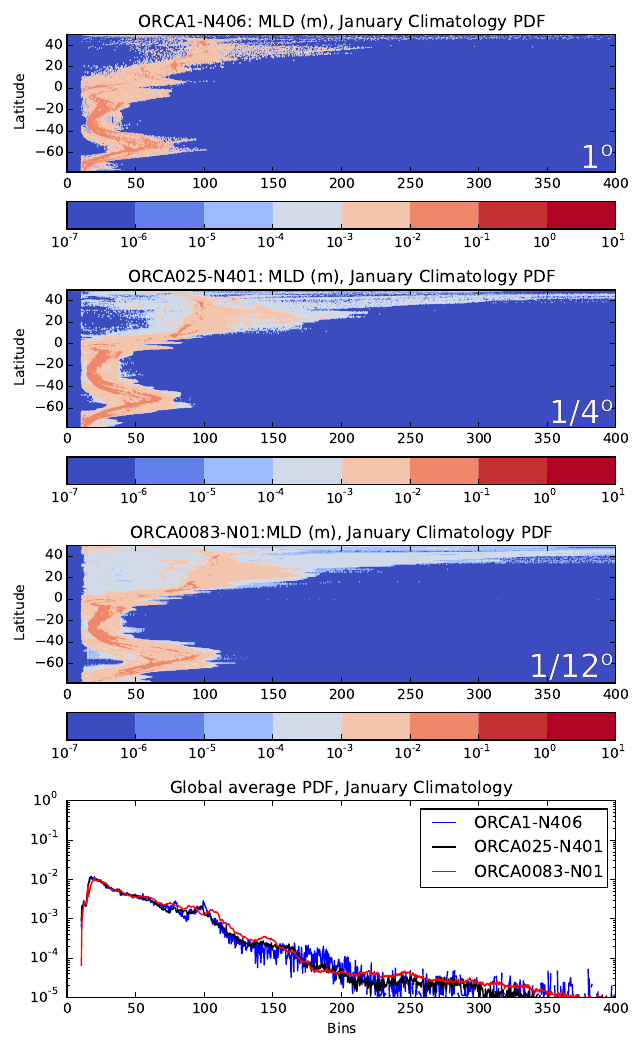
\includegraphics[width=0.4\textwidth]{PDF_MLD_JanCutP.png}
	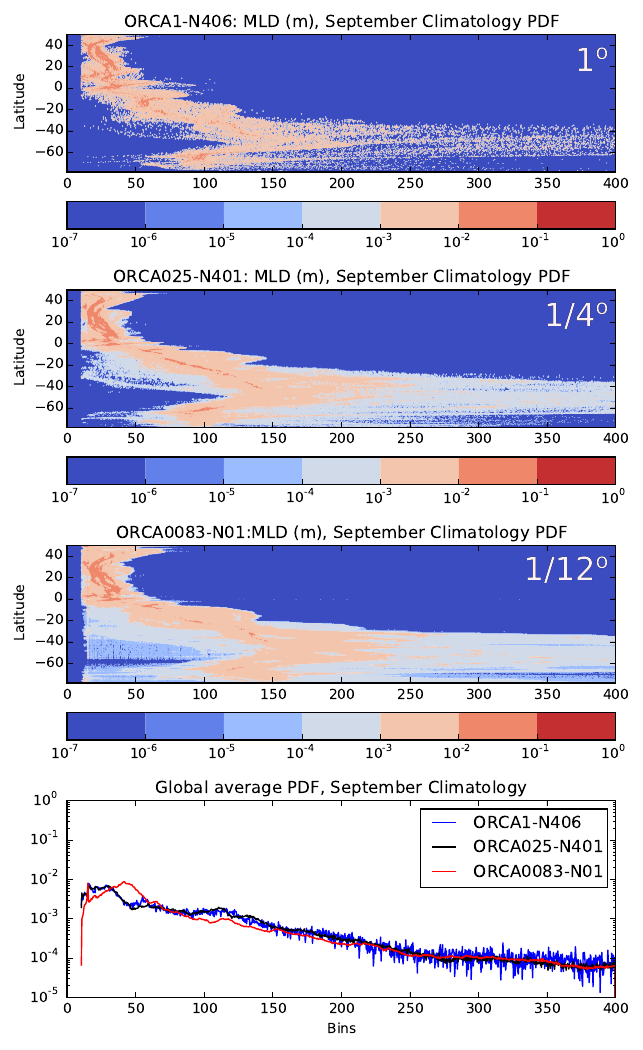
\includegraphics[width=0.4\textwidth]{PDF_MLD_SeptCutP.png}
\end{figure}
\end{frame}


\begin{frame}{Bias: de Boyer Mont\'{e}gut \textit{et al.}, 2004 - NEMO}

\begin{center}
  \LaunchBinary{mld_WOCE_ORCA1_12.avi}{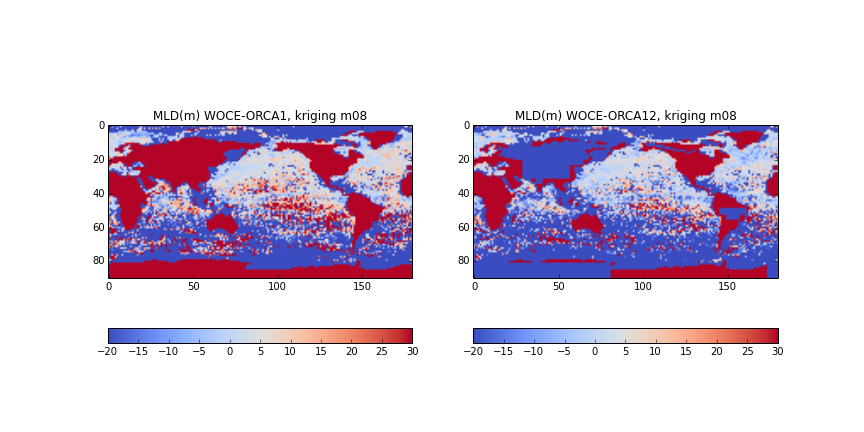
\includegraphics[width=1\textwidth]{mld_WOCE_ORCA1_12_m08.png}}%{Start ORCA12 surface currents}
%\LaunchBinary{/home/maike/Documents/nemo/MLD/WOCE_comp/deBM/mld_deBM.avi}{\includegraphics[width=0.5\textwidth]{/home/maike/Documents/nemo/MLD/WOCE_comp/deBM/mld_deBM_m08.png}}
\end{center}
\end{frame}

\begin{frame}{Surface: Summary}
\begin{itemize}
 \item No significant change in MLD observed
 \item Compares well with observed MLD
\end{itemize}
\pause
\begin{alertblock}{}
 Likely not a place the runs differ greatly in terms of energy pathways
\end{alertblock}
\pause
\begin{itemize}
 \item This and case study of Southern Ocean zonal asymetry: Sonnewald, M., Ferrari, R. and Nurser, A.G., In prep. 
 \item Now on to the interior...
\end{itemize}
% They'ze not that different, now are they..?
\end{frame}


\section{Interior: Steric variability}

\begin{frame}{Steric changes}
%  %equations so ppl know what I'm talking about
 \begin{equation*}
 \eta = \dfrac{1}{\rho_{0}\mathrm{g}}\left( \mathrm{p}_{b}-\mathrm{p}_{a} \right) +\mathrm{SH}
 %\label{bprIsEBSSH}
\end{equation*}
\begin{equation*}
 \mathrm{p_{B}} = \int^{0}_{-H}  \rho \mathrm{g} \mathrm{d}z
%\label{Bpr_gridpoint}
\end{equation*}
 \begin{equation*}
 \mathrm{SH} = -\dfrac{1}{\rho_{0}}\int^{0}_{-H} \rho \mathrm{z}
\end{equation*}
\end{frame}

\begin{frame}{Steric variability}
\begin{equation*}
 SH = \int^{0}_{-H}  \dfrac{\rho_{0}-\rho}{\rho_{0}}\mathrm{d}z
%\label{SH_gridpoint}
\end{equation*}
%\begin{figure}
 % \center
 % \subfloat[Vertical heaving]{\label{vert_heave}
  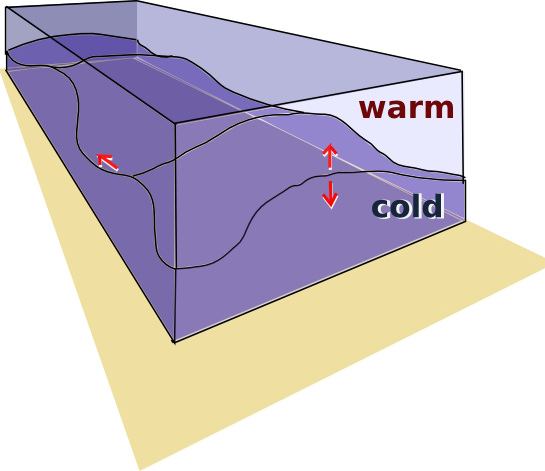
\includegraphics[width=0.5\textwidth]{drawing-1.png}
 % \subfloat[Horizontal meandering]{\label{horiz_meander}
  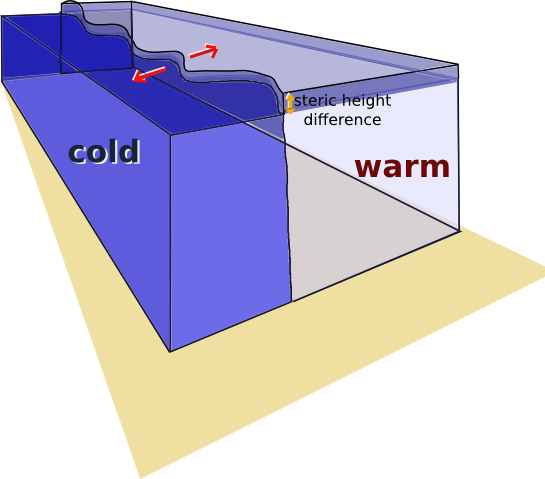
\includegraphics[width=0.5\textwidth]{drawing.png}
  %\caption{\small Schematic illustrating possible causes of steric variability.}
  %\label{drawingsSH}
%\end{figure}
\end{frame}

\begin{frame}{Heaving: What is the deep water water doing?}
\begin{center}
\LaunchBinary{ORCA_twelve_one.mp4}{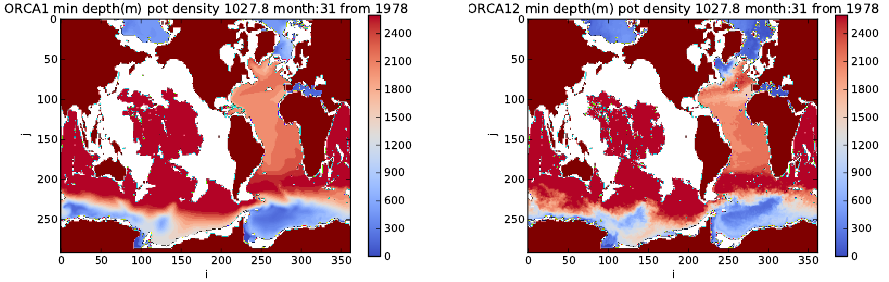
\includegraphics[width=1\textwidth]{rhoDense.png}}%{Start ORCA12 surface currents}
\end{center}
%\LaunchBinary{ORCA_twelve_one.mp4}{Start 1027.8 min depth ORCA1 and ORCA12}
\end{frame}

\begin{frame}{Meandering: What's happening in $\rho$ at 2000m?}
\begin{center}
\LaunchBinary{ORCA_twelve_one_twoThousand.mp4}{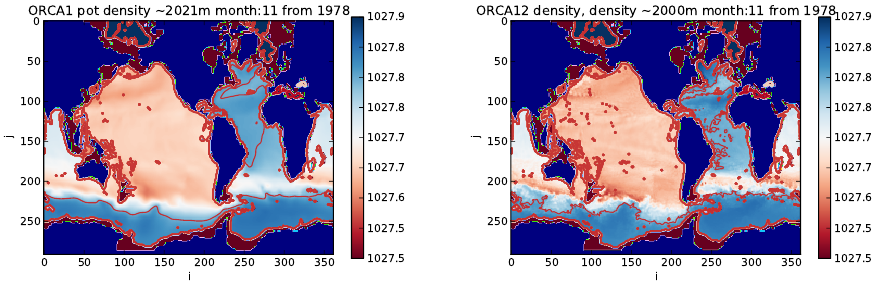
\includegraphics[width=1\textwidth]{rho2000.png}}%{Start ORCA12 surface currents}
\end{center}
\end{frame}




\begin{frame}{Steric variability}
\begin{center}
\vspace{-0.9cm}
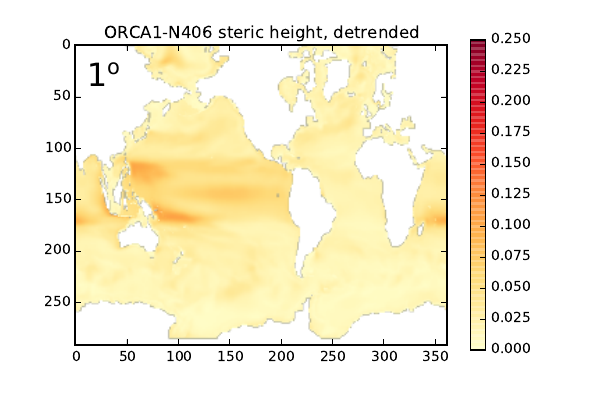
\includegraphics[width=0.55\textwidth]{ORCA1_Std_SH_P.png}
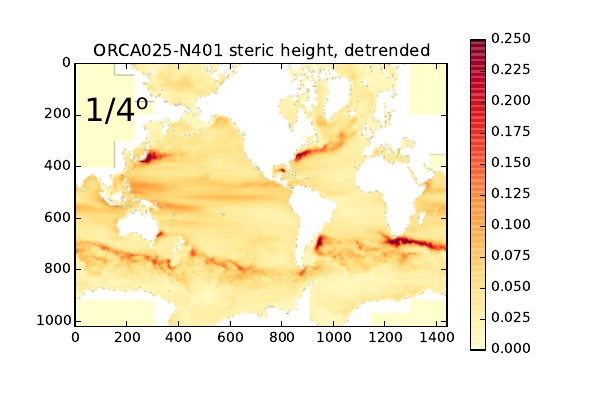
\includegraphics[width=0.55\textwidth]{ORCA025_Std_SH_P.png}\\
\vspace{-0.4cm}

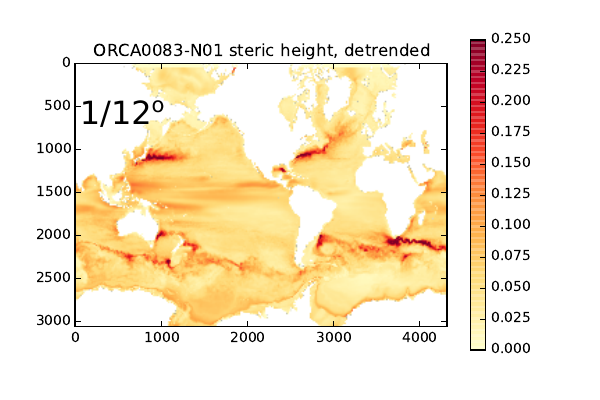
\includegraphics[width=0.5\textwidth]{ORCA12_Std_SH_P.png}
\end{center}
\end{frame}

\begin{frame}{Steric variability PDF}
\vspace{-10}
\begin{center}
 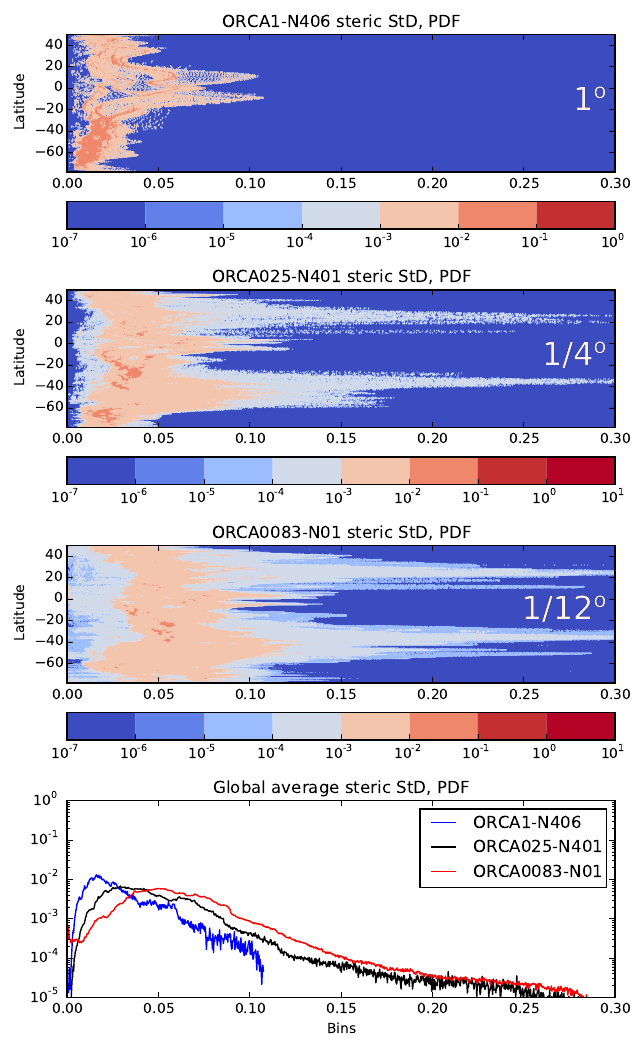
\includegraphics[width=0.4\textwidth]{PDF_SH_stdCutP.png}
\end{center} 
\end{frame}

\begin{frame}{Steric covariance}
\begin{center}
\vspace{-0.9cm}
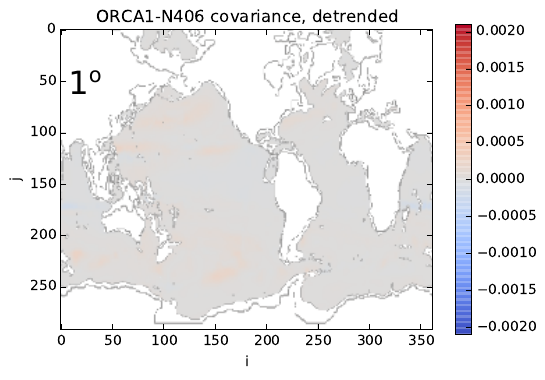
\includegraphics[width=0.5\textwidth]{ORCA1_covP.png}
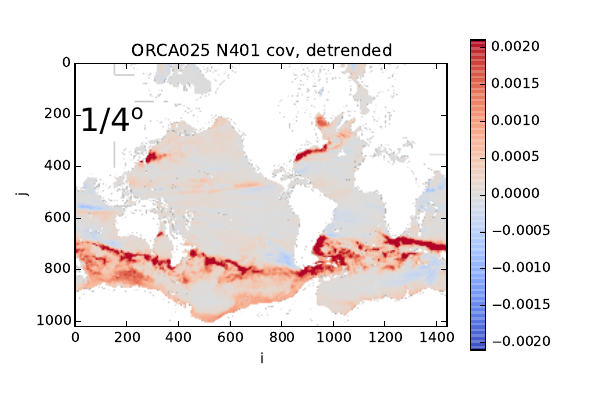
\includegraphics[width=0.55\textwidth]{ORCA025_N401_cov_detrendedMarch2015P.png}\\
\vspace{-0.4cm}
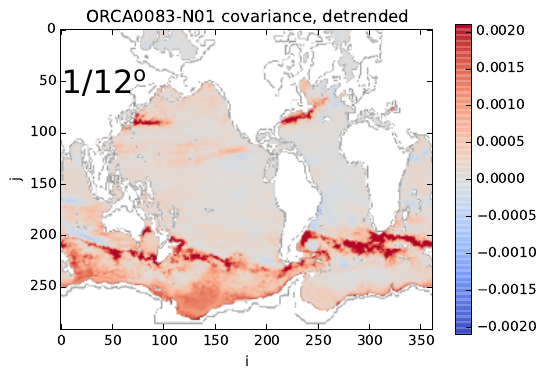
\includegraphics[width=0.5\textwidth]{ORCA12_covP.png}
\end{center}
\end{frame}

\begin{frame}{Steric covariance PDF}
\vspace{-10}
\begin{center}
\centering 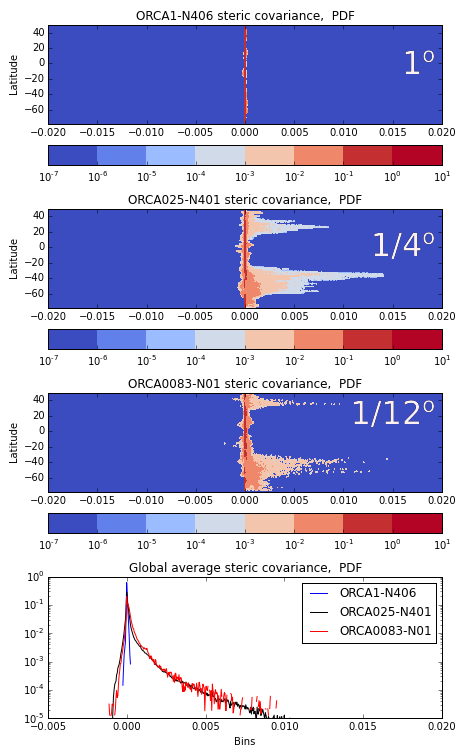
\includegraphics[width=0.4\textwidth]{PDF_SH_covCutP.png}
\end{center} 
\end{frame}

\begin{frame}{Interior: Summary}
\begin{itemize}
 \item Increase in surface<->deep covariance indicates allowing eddy-features changes information exchanges
 \item At 1$^{\circ}$ any covariance is confined to low temporal frequencies
 \item Inviscid assumption:
 \begin{itemize}
  \item Our work does not assess the role of the interior explicitly, but suggests that the adjustement to surface fields could be affected...
 \end{itemize}
\pause
 \item On to the interactions with topography...
\end{itemize}



% They iz pretty different!\\
% Now WTF does that mean?
\end{frame}

\section{Bottom: Bottom Pressure Torque}

\begin{frame}{$\nabla H$: Bathymetry roughness}
\begin{center}
\begin{figure}[H]
\centering
  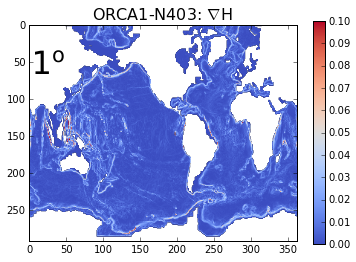
\includegraphics[width=0.4\textwidth]{ORCA1_N403_nablaH_26FebP.png}
  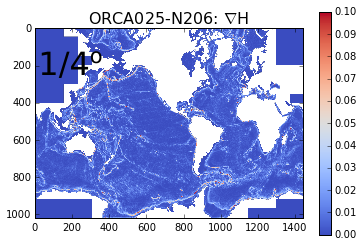
\includegraphics[width=0.45\textwidth]{ORCA025_N206_nablaH_26FebP.png}\\
  \includegraphics[width=0.45\textwidth]{ORCA12_N01_nablaH_26FebP.png}
\end{figure}
\end{center}
\end{frame}

\begin{frame}{Bathymetry interactions:\\Change in the balance of forces?}
%Changing baroclinic contribution suggests a change in the balance of forces.\\

Conserving PV, wind driven gyre sees vorticity innput balanced by flow over f/H contours:
\begin{center}
$$\beta \psi_{x}=\overbrace{-f w_{B}}^{\text{bottom velocity}}+\underbrace{\nabla \times \tau}_{\text{wind stress}} + \overbrace{R'}^{\text{Non-lin terms}}$$
%$$ \beta \psi_{x}=-f w_{B}+\nabla x \tau + R'$$
\end{center}
The link between H and vortex stretching:
$$w_{B} = u_{B}\cdot \nabla (H) \approx \frac{1}{\rho_{0}f}J(p_{B}, H)$$
% \begin{alertblock}{}
% \centering Can illustrate where energy is dissipated?
% \end{alertblock}
\end{frame}


\begin{frame}{Bottom pressure torque ($J(p_{B}, H)$)}
\begin{center}
\begin{figure}[H]
\centering
\vspace{-0.1cm}
\includegraphics[width=0.5\textwidth]{ORCA1_N406_bottom_torqueMeanP.png}
\includegraphics[width=0.5\textwidth]{ORCA025_N401_bottom_torqueMeanP.png}\\
\vspace{-0.15cm}
\includegraphics[width=0.5\textwidth]{ORCA12_N01_bottom_torque_MeanP.png}
\end{figure}
\end{center}
\end{frame}

\begin{frame}{$J(p_{B}, H)$ PDF}
\begin{center}
\begin{figure}[H]
\centering
\centering \includegraphics[width=1\textwidth]{talkPDFmeanBPT_P.png}
\end{figure}
\end{center}
\end{frame}

%\subsection{Baroclinic contribution: JEBAR}
\begin{frame}{Baroclinic contribution to bathymetry interaction: JEBAR}
%Summary from the plot above
$J(p_{B}, H)$ does not seem to account for the change in $\psi$?
\pause
\large
\begin{center}
\begin{equation*}
\dfrac{1}{\rho_{0}} J(p_{B}, H) = f \textbf{v}_{gb} \cdot\bigtriangledown H = \overbrace{H(JEBAR)}^{\text{Baroclinic}}+\overbrace{f\overline{\textbf{v}}_{g} \cdot\bigtriangledown H}^{\text{Barotropic}}
\end{equation*}
\end{center}
\begin{flushright}
\tiny Mertz and Wright (1992)
\end{flushright}
\end{frame}

\begin{frame}{Baroclinic bathymetry interaction: JEBAR}
\begin{center}
\begin{figure}[H]
\centering
\vspace{-0.1cm}
\includegraphics[width=0.5\textwidth]{ORCA1_N406_JEBAR_scientificNotation_P.png}
\includegraphics[width=0.5\textwidth]{ORCA025_N401_JEBAR_scientificNotation_P.png}\\
\vspace{-0.15cm}
\includegraphics[width=0.5\textwidth]{ORCA12_N01_JEBAR_scientificNotation_P.png}
\end{figure}
\end{center}
\end{frame}

\begin{frame}{Baroclinic bathymetry interaction: JEBAR PDF}
\vspace{-15}
\begin{center}
%\begin{figure}[H]
\centering
\includegraphics[width=1\textwidth]{presentationJEBAR_P.png}
%\end{figure}
\end{center}
\pause
\begin{alertblock}{}
\centering We see a large change in the distribution with resolution
\end{alertblock}
\end{frame}

%\section{Conclusion}
\begin{frame}{Summary: topography}
 \begin{itemize}
  \item Stronger baroclinic contribution to overturning with resolution
  \item This happens mainly through changes in bathymetry interactions: JEBAR
  \item Scotia ridge and Kuroshio case studies and further details: Sonnewald, M., Nurser, A.G. and Hirschi, J.J.-M. In Prep.
 \end{itemize}
 \pause
\begin{alertblock}{}
\centering
 \alert{Change in energy dissipation happens baroclinically at depth}
\end{alertblock}

\begin{itemize}
 \item Summarise our results for NEMO in terms of their ``utility''
\end{itemize}
\end{frame}

\section{Utility}
\begin{frame}{Tools for comparing the model runs: Utility}
We explore ``utility'' using notional functions:
 \begin{itemize}
  \item Accuracy (A):                     $\mathrm{\mathbf{A}} = 100 - |\sigma_{EOFbaseline}-\sigma_{EOFmodel}|^{c}$
  \item Analysis inconvenience (I): 	$\mathrm{In} = -0.2x^{-1}ln\left(\frac{2}{x}\right)$
  \item Storage space (S):			 $\mathrm{S} = -4x+5$
  \item Computational cost (C):               		$\mathrm{C} = -0.4x^{-1}$
 \end{itemize}
\begin{alertblock}{}
 \centering $\mathrm{Utility} = \mathrm{\mathbf{A}} + \left( \mathrm{In} + \mathrm{C} + \mathrm{S}\right)\mathrm{I}$
\end{alertblock}
\centering \includegraphics[width=0.5\textwidth]{elementsOfUtility.pdf}
\end{frame}

\begin{frame}{Utility: SST}
\vspace{-0.5cm}
\centering \includegraphics[width=0.9\textwidth]{SSTUtility_1_2_3_P.png}
\end{frame}

\begin{frame}{Utility: SST}
\centering \includegraphics[width=0.9\textwidth]{SST_EOFCut2.png}
\end{frame}
\begin{frame}{Utility: $\psi(\sigma, y)$}
\vspace{-0.5cm}
\centering \includegraphics[width=0.9\textwidth]{mocsigUtility1_2_3_P.png}
\end{frame}

\begin{frame}{Utility: $\psi(\sigma, y)$}
\centering \includegraphics[width=0.9\textwidth]{mocsigF_EOF_Cut2.png}
\end{frame}

\begin{frame}
 \includegraphics[width=1\textwidth]{UtilityCut.pdf}
\end{frame}




\begin{frame}{Conclusion and further work}

\begin{itemize}
  \item The changes in utility in NEMO highlight that certain fields are well captured even at low resolution (MLD) while others require higher resolution. 
  \item We see main changes through interactions with topography and eddy activity
  %\item \alert{I'm not entirely sure how explicit to be...!}
  \item Finite-time Lyapunov exponents (FTLE) also explored, look at contributions to the overturning..?
\end{itemize}

 \pause
\begin{alertblock}{Take home message}
\centering Choices of modeling tools bias results, considering changes in ``utility'' can aid comparison and focus efforts
 %\alert{Take home message}
\end{alertblock}
\end{frame}


\begin{frame}{Selected references:}
\tiny
-Brodeau, L., Barnier, B., Treguier, A.M., Penduff, T. and Gulev, S.: An ERA40-based atmospheric forcing for global ocean circulation models, Ocean Modelling, 31 (3-4), 88-104, 2010.\\
-Madec, G.: NEMO ocean engine, Note du Pole de modélisation, Institut Pierre-Simon Laplace (IPSL), 27, 2008.\\
-Marzocchi, A., Hirschi, J.J.M., Penny, H.N., Cunningham, S.A., Blaker, A.T. and Coward, A.C.: The North Atlantic subpolar circulation in an eddy-resolving global ocean model, Journal of Marine Systems, 142, doi:126-143. 10.1016/j.jmarsys.2014.10.007, 2015.\\
-Jackson, L., Hughes, C.W. and Williams, R.G.: Topographic Control of Basin and Channel Flows: The Role of Bottom Pressure Torques and Friction, J. Phys. Oceanogr., 36, 1786-1805. doi: \url{http://dx.doi.org/10.1175/JPO2936.1}, 2006.\\
-Hughes, C.W.; de Cuevas, B.A.. 2001 Why western boundary currents in realistic oceans are inviscid: a link between form stress and bottom pressure torques. Journal of Physical Oceanography, 31 (10). 2871-2885. doi: \url{http://dx.doi.org/10.1175/1520-0485(2001)031<2871:WWBCIR>2.0.CO;2}\\
-Yeager, S. 2015: Topographic coupling of the Atlantic overturning and gyre circulations. J. Phys. Oceanogr., 45, 1258-1284. doi: \url{http://dx.doi.org/10.1175/JPO-D-14-0100.1}\\

\pause
\vspace{20}
\huge
\begin{centering}
\centering \textcolor{red}{Thank you!}
\end{centering} 

\end{frame}

%Streamfunction


% 
% 
% 
% 
% 
%\section{Zonally cumulative density space overturning}

\begin{frame}{Model grid: Surface volume (m$^{3}$)}
\begin{center}
\includegraphics[width=0.5\textwidth]{ORCA1_surfVol.pdf}
\includegraphics[width=0.5\textwidth]{ORCA025_surfVol2.png}\\
\vspace{-0.4cm}
\includegraphics[width=0.5\textwidth]{ORCA12_surfVol.pdf}
\end{center}
\end{frame}

\begin{frame}{Cumulative density transport 57S: ORCA1}
\begin{center}
\LaunchBinary{cumDenTranspORCA1-N406_t_060.avi}{\includegraphics[width=1\textwidth]{cumDenTranspORCA1-N406_t_060_t_000.png}}%{Start ORCA12 surface currents}
\end{center}
\end{frame}

\begin{frame}{Cumulative density transport 57S: ORCA12}
\begin{center}
\LaunchBinary{cumDenTranspORCA12_fast.avi}{\includegraphics[width=1\textwidth]{cumDenTranspORCA12_t_000.png}}%{Start ORCA12 surface currents}
\end{center}
\end{frame}

\begin{frame}{Cumulative density transport 57S: ORCA1 barotropic}
\begin{center}
\LaunchBinary{cumDenTranspORCA1-N406_barot_060.avi}{\includegraphics[width=1\textwidth]{cumDenTranspORCA1-N406_barot_t_060_t_000.png}}%{Start ORCA12 surface currents}
\end{center}
\end{frame}

\begin{frame}{Cumulative density transport 57S: ORCA1 baroclinic}
\begin{center}
\LaunchBinary{cumDenTranspORCA1-N406_baroc_060.avi}{\includegraphics[width=1\textwidth]{cumDenTranspORCA1-N406_baroc_t_060_t_000.png}}%{Start ORCA12 surface currents}
\end{center}
\end{frame}

%\section{Utility results}

\begin{frame}{How do we interpret this...?}
  \begin{center} \includegraphics[width=1\textwidth]{rhoInfoGraphic.png}\end{center}
\end{frame}

\begin{frame}{gradH PDF}
  \begin{center} \includegraphics[width=0.35\textwidth]{PDF_H.png}\end{center}
\end{frame}

\begin{frame}
\center
\includegraphics[width=0.5\textwidth]{accMass_take2.png}\\
\includegraphics[width=0.5\textwidth]{accMassORCA025_N401.png}
\includegraphics[width=0.5\textwidth]{accMassORCA0083.png}
\end{frame}

\begin{frame}{Transport section}
\begin{center}
\LaunchBinary{ORCA1_12_fullZonalVel_60.avi}{\includegraphics[width=1\textwidth]{mergedORCA12_fullZonalVel_60_t000.png}}%{Start ORCA12 surface currents}
\end{center}
%\LaunchBinary{mocsigORCA1_12_barot.avi}{Start Barotropic density space overturning ORCA1 and ORCA12}
\end{frame}





% 
% 
% \begin{frame}
%  \begin{figure}[H]
%  \vspace{-25}
% \centering
%   \subfloat[ORCA0083-N01 mean, barotropic]{\label{mocsig12MeanBarot}\includegraphics[width=0.3\textwidth]{/home/maike/Documents/thesis/overturning/mocsigORCA12MeanBarot.png}}
%   \subfloat[ORCA0083-N01 mean, baroclinic]{\label{mocsig12MeanBaroc}\includegraphics[width=0.3\textwidth]{/home/maike/Documents/thesis/overturning/mocsigORCA12MeanBaroc.png}}\\
%   \subfloat[ORCA025-N401 mean, barotropic]{\label{mocsigJan025}\includegraphics[width=0.3\textwidth]{/home/maike/Documents/thesis/overturning/mocsigORCA025_barot_mean.png}}
%   \subfloat[ORCA025-N401 mean, baroclinic]{\label{mocsigJun025}\includegraphics[width=0.3\textwidth]{/home/maike/Documents/thesis/overturning/mocsigORCA025_baroc_mean.png}}\\
%   \subfloat[ORCA1-N406 mean, barotropic]{\label{mocsigJan1}\includegraphics[width=0.3\textwidth]{/home/maike/Documents/thesis/overturning/mocsigORCA1_N406_barot_Mean.png}}
%   \subfloat[ORCA1-N406 mean, baroclinic]{\label{mocsigJun1}\includegraphics[width=0.3\textwidth]{/home/maike/Documents/thesis/overturning/mocsigORCA1_N406_baroc_Mean.png}}
%   \caption{\normalsize The overturning in $\rho$ space. Showing the mean barotropic and baroclinic circulation from the 1978 to 2007 timeseries.}
%   \label{mocsigBarotBaroc}
% \end{figure}
%  
% \end{frame}
% 
% \begin{frame}
%  \vspace{-25}
%   \begin{figure}[H]
% \centering
%   \subfloat[ORCA0083-N01 StD, barotropic]{\label{mocsig12StDBarot}\includegraphics[width=0.3\textwidth]{/home/maike/Documents/thesis/overturning/mocsigORCA12StDBarot.png}}
%   \subfloat[ORCA0083-N01 StD, baroclinic]{\label{mocsig12StDBaroc}\includegraphics[width=0.3\textwidth]{/home/maike/Documents/thesis/overturning/mocsigORCA12StDBaroc.png}}\\
%   \subfloat[ORCA025-N401 StD, barotropic]{\label{mocsigJan025}\includegraphics[width=0.3\textwidth]{/home/maike/Documents/thesis/overturning/mocsigORCA025_barot_StD.png}}
%   \subfloat[ORCA025-N401 StD, baroclinic]{\label{mocsigJun025}\includegraphics[width=0.3\textwidth]{/home/maike/Documents/thesis/overturning/mocsigORCA025_baroc_StD.png}}\\
%   \subfloat[ORCA1-N406 StD, barotropic]{\label{mocsigJan1}\includegraphics[width=0.3\textwidth]{/home/maike/Documents/thesis/overturning/mocsigORCA1_N406_barot_StD.png}}
%   \subfloat[ORCA1-N406 StD, baroclinic]{\label{mocsigJun1}\includegraphics[width=0.3\textwidth]{/home/maike/Documents/thesis/overturning/mocsigORCA1_N406_baroc_StD.png}}
%   \caption{\normalsize The overturning in $\rho$ space. Showing the StD barotropic and baroclinic circulation from the 1978 to 2007 timeseries.}
%   \label{mocsigBarotBaroc}
% \end{figure}
% \end{figure}
%  
% \end{frame}


%\section{Overturning}
\begin{frame}{Overturning: Density space}
\begin{center}
\LaunchBinary{mocsigORCA1_12_full_short.avi}{\includegraphics[width=1\textwidth]{mergedmocsigORCA12_full_300.png}}%{Start ORCA12 surface currents}
\end{center}
\end{frame}
% 
%Baroclinic
\begin{frame}{Density space overturning: Baroclinic}
\begin{center}
\LaunchBinary{mocsigORCA1_12_baroc_short.avi}{\includegraphics[width=1\textwidth]{mergedmocsigORCA12_baroc_300.png}}%{Start ORCA12 surface currents}
\end{center}
%\LaunchBinary{mocsigORCA1_12_baroc.avi}{Start Baroclinic density space overturning ORCA1 and ORCA12}
\end{frame}
%Barotropic
\begin{frame}{Density space overturning: Barotropic}
\begin{center}
\LaunchBinary{mocsigORCA1_12_barot_short.avi}{\includegraphics[width=1\textwidth]{mergedmocsigORCA12_barot_300.png}}%{Start ORCA12 surface currents}
\end{center}
\end{frame}

\begin{frame}{ORCA1-N406: Climatology 1978-2007}
\begin{center}
\LaunchBinary{mocsigORCA1_N406_full_clim.avi}{\includegraphics[width=1\textwidth]{mocsigORCA1_N406_full_clim1.png}}%{Start ORCA12 surface currents}
\end{center}
\end{frame}

\begin{frame}{ORCA025-N401: Climatology 1978-2007}
\begin{center}
\LaunchBinary{mocsigORCA025_fullClim_.avi}{\includegraphics[width=1\textwidth]{mocsigORCA025_fullClim_1.png}}%{Start ORCA12 surface currents}
\end{center}
\end{frame}


\end{document}
